\section{Module 6. Diffusion tensor imaging}

\textbf{Preprocessing and Module I/O}

In order to improve diffusion tensor estimation it is imperative to
remove artifacts. In addition to standard MRI pre-processing, one
needs to correct for artifacts arising the use of diffusion-gradient
pulse sequences and longer acquisition time. While hardware manufacturers
try to proactively diminish some of these effects, software processing
is still mandatory. 
\hfill\\

\textbf{Module Input}:
\begin{itemize}
	\item 
	3D structural data array of shape X x Y x Z, where XY - pixel image intensities, Z - chosen slice, which is the T1- or T2-weighted image corresponding the the given DWI acquisition
	
	\item 
	4D diffusion data array of shape X x Y x Z x M, where XY - pixel image intensities, Z - chosen slice, M - applied diffusion gradient direction
	
	\item 
	b\_value, a scalar value corresponding to applied diffusion gradient sequence magnitude
	
	\item 
	2D gradients matrix of shape M x 3, where each row corresponds to a normalized $(x,y,z)$ components of diffusion gradient sequence vectors
		
	\item 
	optionally - 3D binary mask of shape X x Y x Z, corresponding to the brain area detected by Module 8 (Skull Stripping); if not supplied, DTI is computed on each input data voxel

\end{itemize}
\hfill

\textbf{Module Output}:
\begin{itemize}
	\item
	list of size Z, corresponding to each slice; every list element is a dictionary of biomarker images: MD, RA, FA, VR of shape X x Y, and biomarker FA\_rgb of shape X x Y x 3
\end{itemize}

\subsection{Initialization}

In order to abstract DTI implementation from end-user, all classes and methods other than the main function \texttt{run\_module} are private to module source code script. It is important to note that prior to running the module one has to provide the module with input data object, as well as SOLVER and FIX\_METHOD parameters. SOLVER passed as an argument decides whether to use WLS or NLS estimation, whole FIX\_METHOD decides how to "fix" negative eigenvalues. 

As mentioned in the detailed description chapter, 'ABS' takes absolute value of each eigenvalue, while 'CHOLESKY' ensures that the estimated tensor is positive definite. Eigenvalues of positive definite matrices are always non-negative. 'ABS' is a post-estimation fix, meaning that it does not modify the default estimation algorithm (i.e. it is applied after WLS or NLS computation), while 'CHOLESKY' directly modifies the expressions for WLS and NLS cost function gradients and Hessian matrices.

After passing all required arguments to the \texttt{run\_module} function, they are reshaped internally in order to be compatible with module. Concretely, \texttt{DTISolver} class instance, computing the DTI proper, assumes that input data argument is a concatenated 3D array of both structural and diffusion images, which are stored separately in the original data structure. Moreover, b\_value and gradient fields are reshaped to be lists correpsonding to each slice of the new data array (that is: b\_value is repeated in length while both have zeros appended that correspond to structural images). Finally, all of the above is done separately for each slice and DTI module performs it's computation slice-by-slice due to memory constraints.

\subsection{WLS-ABS estimation}

WLS with the ABS fix method is the fastest yet simple method of module pipeline computation based on diffusion tensor estimation. As such these parameters were set as default for DTI.

Diffusion tensor estimate was computed by implementing the equation:
\begin{equation}
\begin{aligned}
\boldsymbol{\gamma}=\left(\boldsymbol{W}^T\boldsymbol{\omega}^T\boldsymbol{\omega}\boldsymbol{W}\right)^{-1}\boldsymbol{W}^T\boldsymbol{\omega}^T\boldsymbol{\omega y}
\end{aligned}
\label{Eq:m6_impl_eq_1}
\end{equation}

using NumPy matrix broadcasting operations, effectively abstracting away array reshaping. Weights vector $\boldsymbol{\omega}$ is calculated using a separate function in order to avoid changing every piece of code refering to WLS weights in case they change. The following implementation assumes the simplest of models presented in the Detail Description chapter, that is weights being equal to the measured signal.

\subsection{NLS-ABS estimation}

In case of NLS estimation, in addition to implementing gradient and Hessian matrix computation methods:

\begin{equation}
\begin{aligned}
\nabla{f_{NLS}}&=-\boldsymbol{W}^T\boldsymbol{\hat{S}}\boldsymbol{r} \\
\nabla^2{f_{NLS}}&=\boldsymbol{W}^T\left(\boldsymbol{\hat{S}^T\hat{S}-\boldsymbol{R\hat{S}}}\right)\boldsymbol{W}
\end{aligned}
\label{Eq:m6_impl_2}
\end{equation}

It is important to devise an iterative scheme because gradient result depends on NLS diffusion tensor estimate. For that reason an algorithm based on \cite{m6_koay2006a} has been implemented. The method itself is called a Modified Newton's Algorithm and can be summarised as in Fig.\ref{fig:m6_pic_1}.

\begin{figure}[H]
	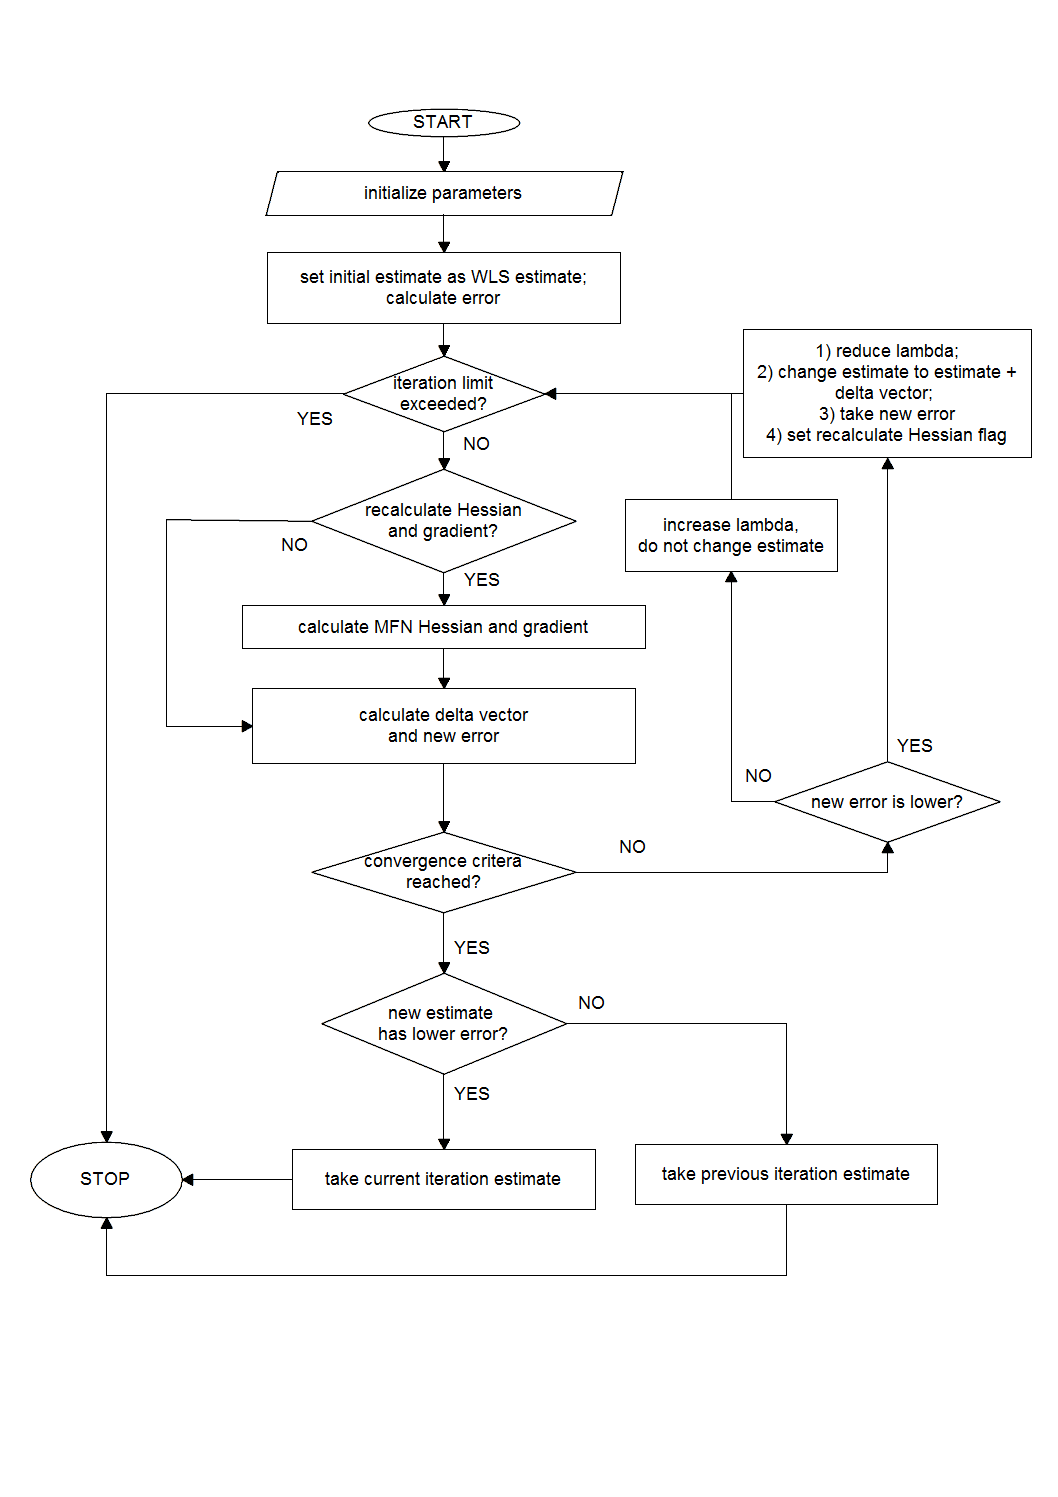
\includegraphics[width=8cm]{figures/Module_06/mfn_simple}
	\centering
	\caption{Modified Newton's method for iterative computation of NLS estimate \vbox{(based on \cite{m6_koay2006a})}}.
	\label{fig:m6_pic_1}
\end{figure}

The following parameters (collectively known in code as MFN parameters) were set:
\begin{itemize}
	\item 
	MFN\_MAX\_ITER = 3 - iteration limit
	
	\item
	MFN\_ERROR\_EPSILON = 1e-5 - first convergence criterion (error change is small)
	
	\item
	MFN\_GRADIENT\_EPSILON = 1e-5 - second convergence criterion (vanishing gradient)
	
	\item
	MFN\_LAMBDA\_MATRIX\_FUN = 'identity'- regularization matrix added to Hessian matrix
	
	\item 
	MFN\_LAMBDA\_PARAM\_INIT = 1e-4 - initial regularization matrix multiplier
\end{itemize}

Delta estimate is calculated from the following formula:
\begin{equation}
\boldsymbol{\delta}=-\left(\nabla^2{f_{NLS}+\lambda I}\right)^{-1}\nabla{f_{NLS}}
\label{Eq:m6_impl_3}
\end{equation}
